\chapter{Design}\label{ch:design}

This section discusses the design of the system. The first part explains query
spawning and execution, the second part describes how data stream can be shared
between queries.

\section{Overall Architecture}

Our system consists of multiple components which are briefly described in this
paragraph. A dataflow program submitted to run as part of the system is
called a \emph{query}. Following Timely's terminology, the execution of a query
is done by a group of \emph{worker} threads. Each worker manages the scheduling and
notification of the nodes that are part instance of the dataflow graph.

A query is executed by one or more \emph{executors}. Each executor selected to
execute a query will fetch and invoke the query binary, ulimately spawning the
worker threads.

All these components are managed by a central process called the
\emph{coordinator}. To achieve this, the coordinator hosts the \emph{catalog}, a
datastructure which contains all information about the available executors, the
running queries and their workers.

\begin{figure}[h]
  \centering
    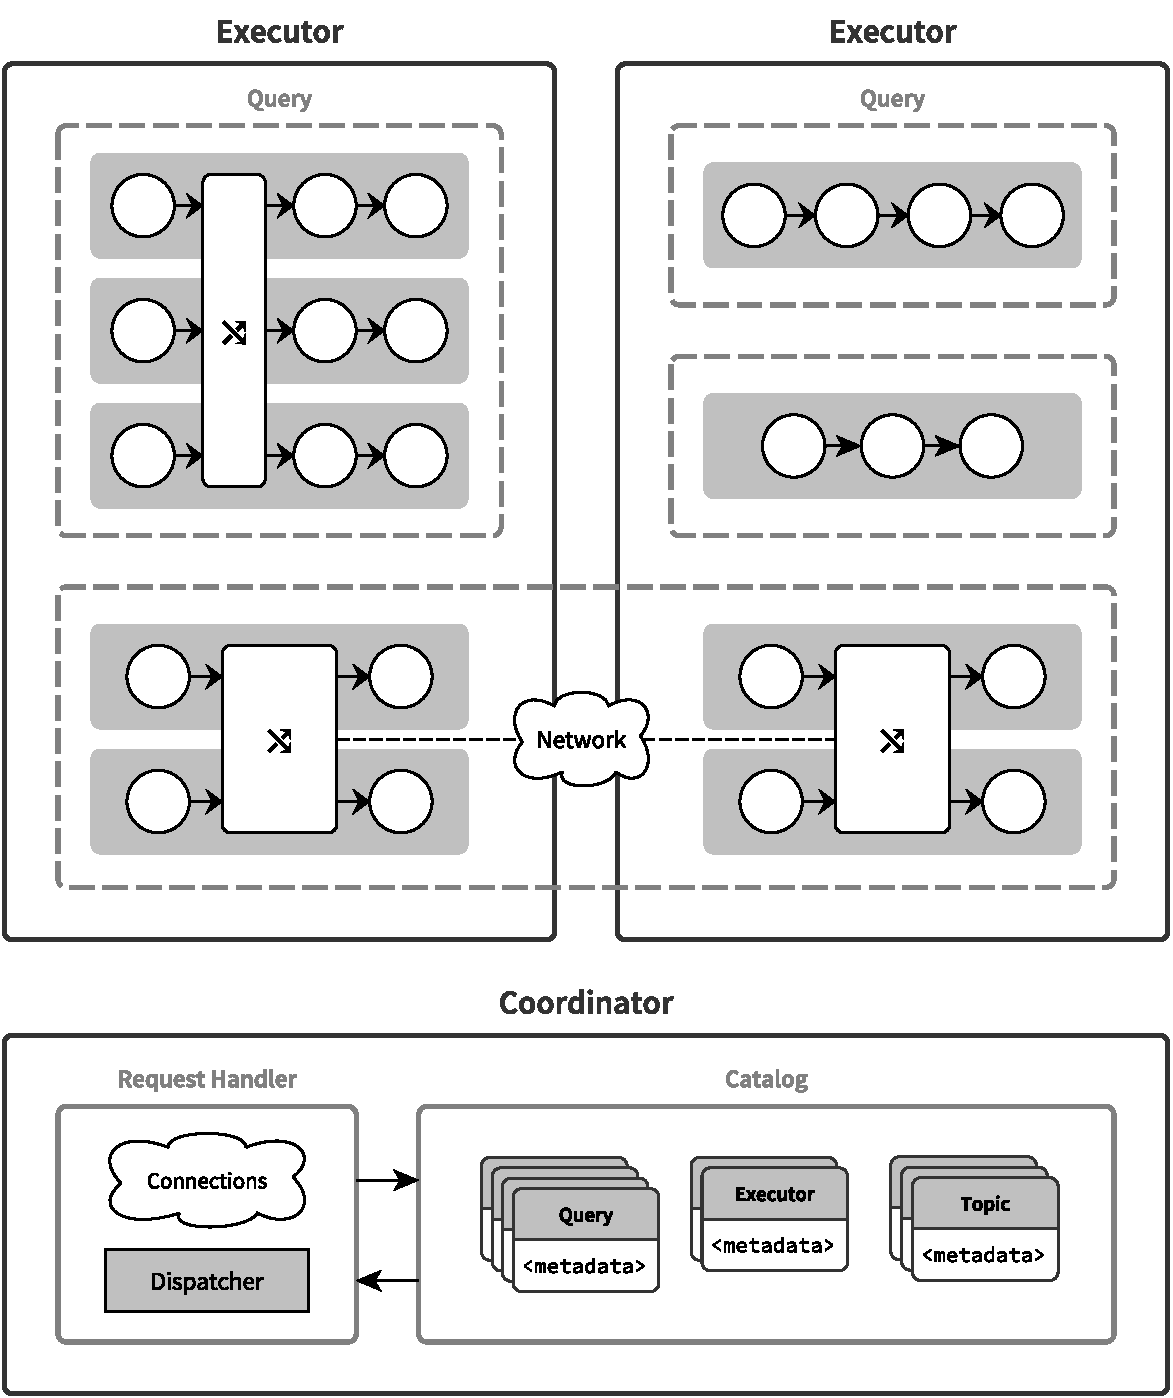
\includegraphics[width=1\textwidth]{figures/components}
  \caption{System overview.}
  \label{fig:components}
\end{figure}

\section{Queries}

A query is a Timely Dataflow program managed and executed by our system. Like
standalone Timely Dataflow programs, queries are written in Rust by using the
Timely Dataflow library: The dataflow graph is constructed by connecting
Timely's operators (vertices) to stream objects (edges).

In order for a Timely Dataflow program to become runnable on the system, it needs
to register its computational logic with with our system library instead of
using one of Timely Dataflow's \texttt{execute} functions. This query library
not only performs the initialization for the query, it also provides additional
functions to interact with the catalog.

\subsection{Compilation}

\subsection{Submission}

\section{Communication paradigm}

Pubsub

\section{Execution model}
